% ==============================================================================
% PAGE 25: 9) PERMANENT MAGNET DIRECT CURRENT (PDMC) MOTOR (Numbered Page 17)
% ==============================================================================
\subsubsection*{9) PERMANENT MAGNET DIRECT CURRENT (PDMC) MOTOR}

\begin{center}
  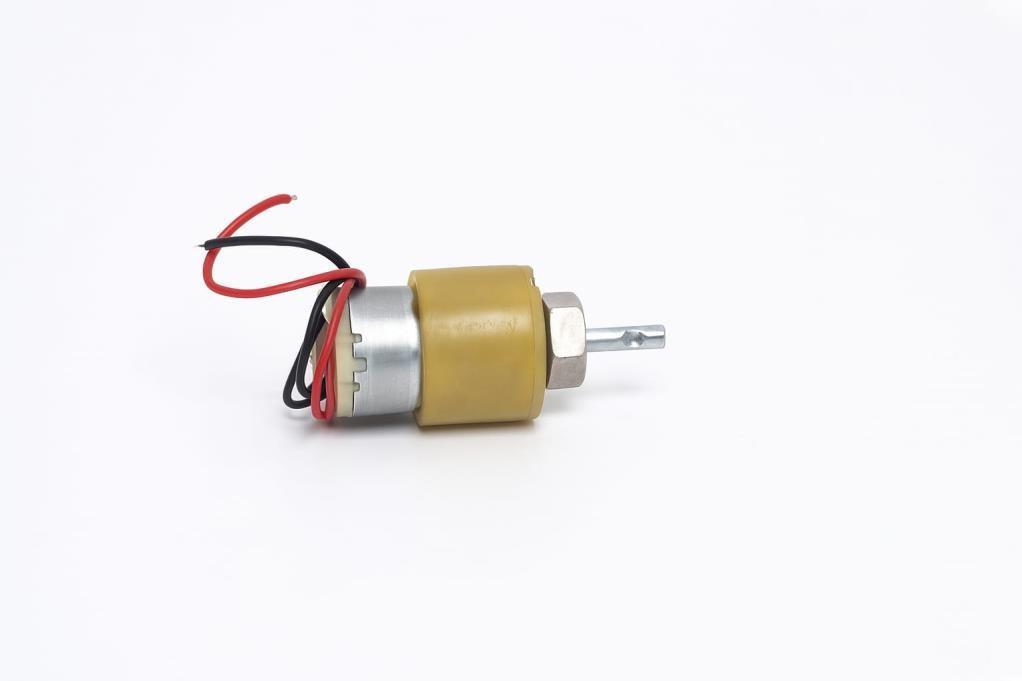
\includegraphics[width=70mm]{figures/fig10_pmdc_motor.jpg}
\end{center}

\noindent
{\fontsize{10.5}{15}\selectfont
\textbf{Specifications}\\[1.5mm]
\textbf{Voltage:} 6V or 9V DC\\[1.5mm]
\textbf{Speed:} 100--300 RPM (depends on load)\\[1.5mm]
\textbf{Power:} 5--15 Watts\\[1.5mm]
\textbf{Control:} Easily reversible by changing polarity\\[3.5mm]
\textbf{Function}\\[2mm]
\textbf{1. Tracking Motion:}\\
The motor is used to rotate the dish (either horizontally or vertically) to follow the sun's movement throughout the day. It ensures maximum solar radiation is focused on the receiver.\\[2.5mm]
\textbf{2. Automatic Control:}\\
The motor operates through a motor driver and sensor system (like LDR sensors) that detect sunlight direction.\\[2.5mm]
\textbf{3. Power Source:}\\
It is powered by a battery or solar panel output, making the system self-sustainable.
}
\clearpage
